\documentclass{amsart}
\usepackage[utf8]{inputenc}
\usepackage[a4paper, total={6in, 8in}, portrait, margin=1in]{geometry}
\usepackage{graphicx}
\usepackage{amsfonts}
\usepackage{amsmath}
\usepackage[toc,page]{appendix}
\usepackage{listings}
\usepackage{float}
\newtheorem{theorem}{Theorem}
\newtheorem{remark}[theorem]{Remark}
\newtheorem{definition}[theorem]{Definition}
\newtheorem{example}[theorem]{Example}
\newtheorem{lemma}[theorem]{Lemma}

\title{Practical Data Science with R - MAT00058H - Homework 2}
\author{Matthew Knowles}
\date{Spring Term, Week 3}

\begin{document}

\maketitle

\section{Corrolations}
We begin by looking at the corrolations of the variables in the dataset. We do this using the \textit{cor()} function, and coerce the resulting object into a matrix by using the \textit{as.matrix()} fucntion.

Seen as this matrix is rather large and hard to read a plethera of numbers, we instead chose to use a heatmap to visualise the corrolations better. In the below figures we see the resulting heatmaps.
\\
\begin{figure}[h]
    \centering
    \begin{minipage}[b]{0.45\textwidth}
        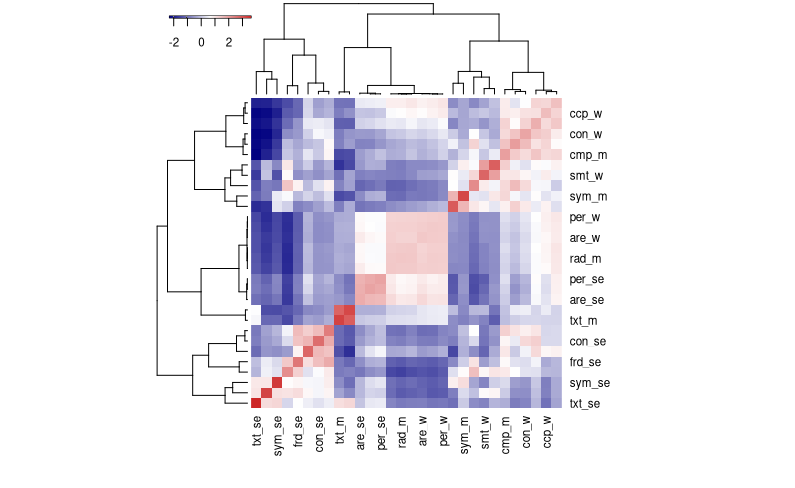
\includegraphics[width=\textwidth]{../../figs/hw2/heatmap1.png}
        \caption{Scaled corrolation heatmap}
    \end{minipage}
    \hfill
    \centering
    \begin{minipage}[b]{0.45\textwidth}
        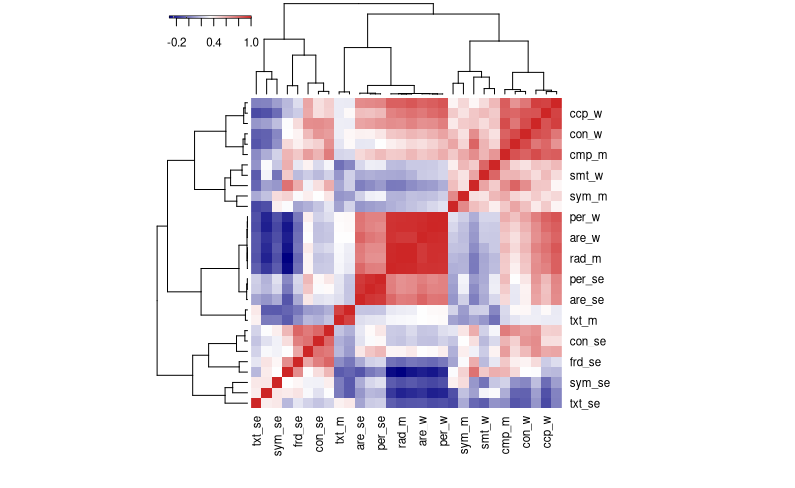
\includegraphics[width=\textwidth]{../../figs/hw2/heatmap2.png}
        \caption{Unscaled corrolation heatmap}
    \end{minipage}
\end{figure}

We can see a lot of lower corrolations, but there appears to be a lot more positive corrolation on the middle variables. This is more pronounced in the unscaled corrolation, as is to be expected.

\section{PCA}
We now move on to some PCA. We begin by taking the data as-is to see how it looks. The biplot for this is seen below.

\begin{figure}[h]
    \centering
    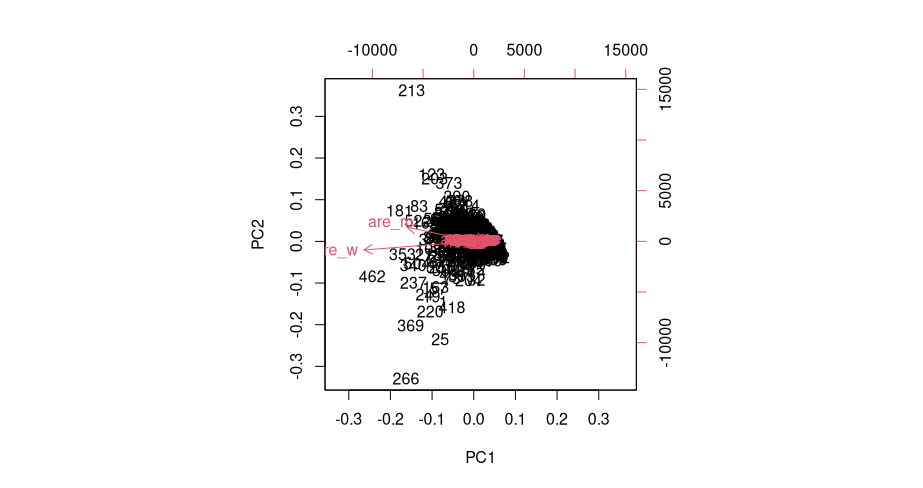
\includegraphics[width=0.85\linewidth]{../../figs/hw2/pcanonscale.png}
    \caption{Biplot for intial PCA- no scaling}
\end{figure}

In this plot we can see that there are 2 data points we may consider to be outliers- 213 and 266. Before deciding whether to remove these and whether or not to scale the data. We produced a boxplot to see which variables are contributing the most to the data.

\begin{figure}[h]
    \centering
    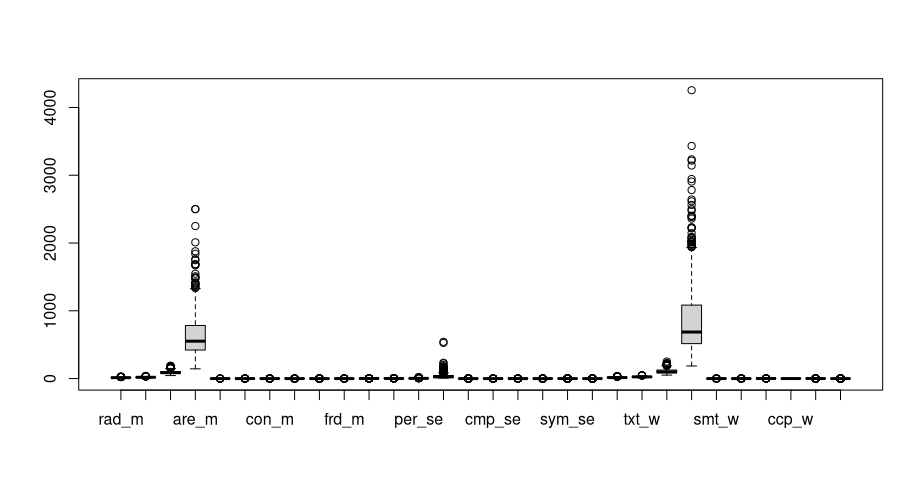
\includegraphics[width=0.8\linewidth]{../../figs/hw2/boxplot.png}
    \caption{Boxplot of variables}
\end{figure}

This shows clearly that the area variable, both in mean and max value is dominating the analysis, so scaling is a wise idea. This gives an updated biplot as follows:

\begin{figure}[h]
    \centering
    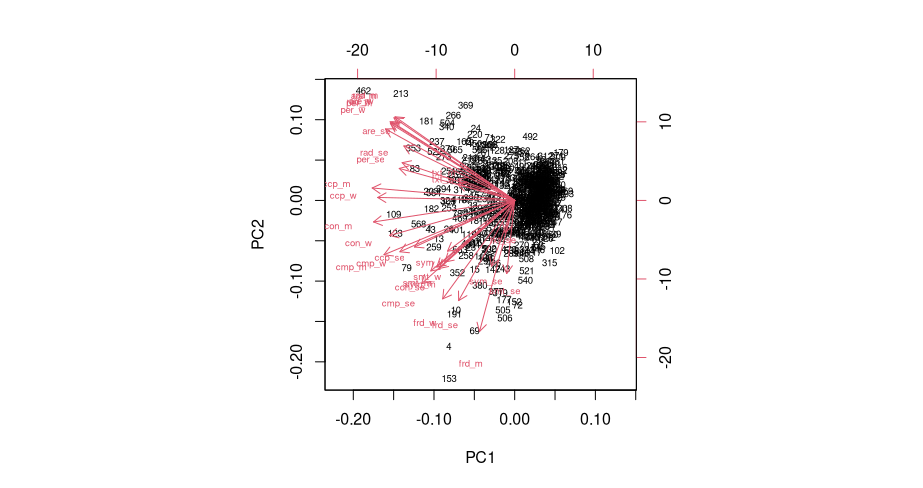
\includegraphics[width=0.8\linewidth]{../../figs/hw2/biplotScaled.png}
    \caption{Scaled biplot}
    
\end{figure}

Now we can see here that there are still some outliers, and 213 is still amongst this crowd. We identify 4, 153, 123 and 462 as outliers, and remove them by creating a new dataset which just leaves them out. This probably isn't the most efficient way to do this, but it works quite nicely. We then finally perform one last PCA to give the following biplot:


\begin{figure}[h]
    \centering
    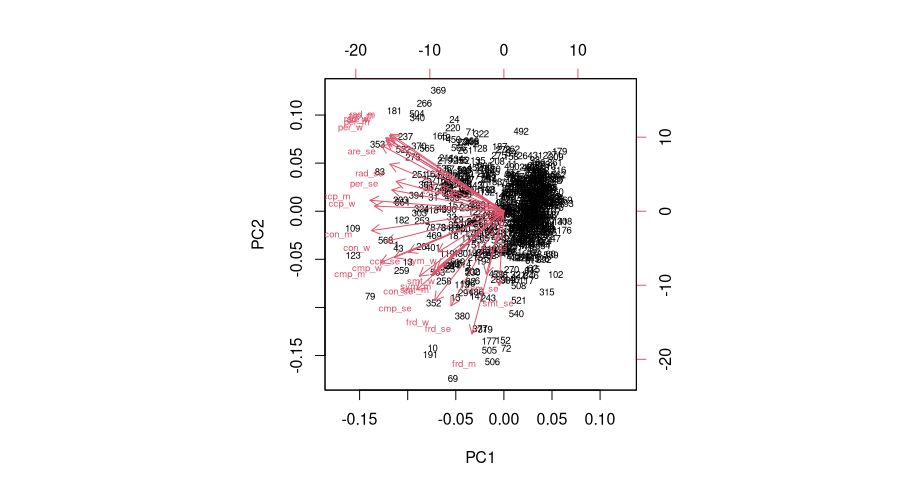
\includegraphics[width=0.8\linewidth]{../../figs/hw2/finalbiplot.png}
    \caption{Biplot of scaled and outlier-free dataset}
\end{figure}

With that sorted we can look at the loadings and the corrolations between them. The heatmap below is produced in an almost identical way to the one earlier.

\\

\begin{figure}[h]
    \centering
    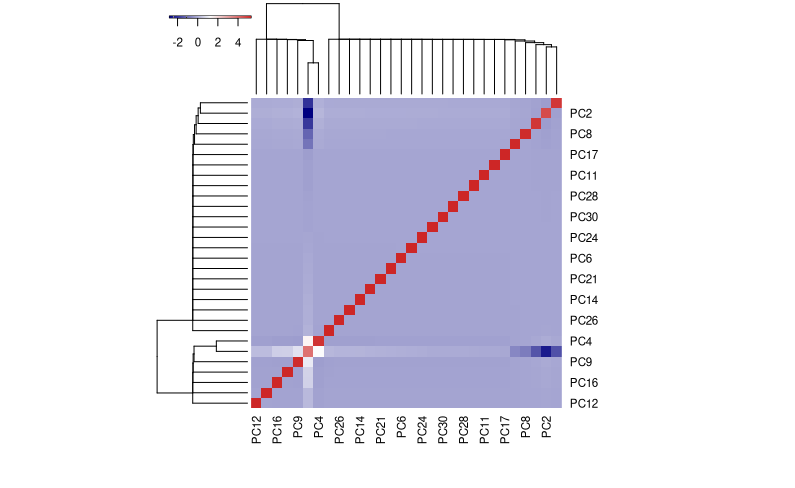
\includegraphics[width=0.8\linewidth]{../../figs/hw2/pcaCorr.png}
    \caption{Corrloation heatmap for Principal Component Loadings}
\end{figure}

\newpage

It can be seen that most of the principal components are not really correlated, however between PC1 and PC9, there is a lot of corrolation going on. By looking at the values in the matirx used to create this heatmap, we find that the corrolation between PC1 and PC2 is $-0.5906$, which is the highest and then for PC1 and PC3 it is roughly  $-0.7372$. Interestingly, PC1 and PC4 are highly positively corrolated, coming in at a value of around  $0.31$.

Considering the above, before performing PCA-LDA I am making the choice to use 6 principal components for the following analysis. This is further supported by using \textit{summary(tumPCAScaled)} which shows us that the first 6 principle components make up 90\% of the total variance.

\section{LDA and L-O-O}

We run through LDA in the standard way, as can be seen in the code given in the appendix.

\\

\begin{center}
    \begin{tabular}{c & c & c}
        $\dot$ & B & M \\
        B & 356 & 0 \\
        M & 29 & 180 
    \end{tabular}
\end{center}

Finally, runnign \textit{sum(diag(prob.table(class)))} which gives us a finally accuracy of 95\% on classification with 6 principal components.

\begin{appendices}
\chapter{R Source Code}
\lstinputlisting[language=R]{../../Rscripts/prac2b.R}
\end{appendices}


\end{document}

